\documentclass[handout,space,nooutcomes]{ximera}
%\documentclass{ximera}

\graphicspath{{./}{eulerCharacteristic}}

%\usepackage[strict]{changepage}

\title{Paying off Debt}
\author{Brad Findell \and Bart Snapp}
\begin{document}
\begin{abstract}
Here we investigate where your payments go when you pay off debt.
\end{abstract}
\maketitle

When you take out a loan, the amount of the loan is called
\textbf{principal}.  For most loans, interest is calculated monthly,
based on an \textbf{annual interest rate}, and based on the remaining
balance.  When you make a payment, your payment first offsets the
accumulated interest and then is applied to principal, in order to
calculate the \textbf{remaining principal balance}.  The loan is paid
back in full when the remaining principal balance is reduced to zero.


Although loans are typically paid monthly, we first explore annual payments to simplify and shorten the calculations.  

\begin{question}
Suppose you borrow $\$6{,}000$ and agree to pay it back in \textbf{equal} annual
payments over $4$ years.  Interest is calculated at $5\%$,
compounded annually. 

Without making any complicated calculations, let's make a guess at what the annual payment should be.  

First, if the interest rate were $0\%$, the payment would need to be $\answer{6000/4}$ dollars in order to pay off the loan in 4 years.  

\begin{question}
Correct!  This can serve as a lower bound for what the annual payment will need to be.  

Before thinking about an upper bound for the annual payment, how much interest will accrue during the year 1 of the loan of $\$6{,}000$ 
at an interest rate of $5\%$?  
$\answer{6000\times.05}$ dollars.  

\begin{question}
Correct!  

And in subsequent years, the accrued interest will be less because the remaining principal balance will be less.  
So adding the year-1 interest to our lower-bound gives a good upper bound of $\answer{1800}$.  
 
\end{question}
\end{question}
\end{question}

\newpage
\begin{question}
We first approach this problem numerically.  Let's \emph{split the difference} (exactly) between our lower- and upper-bounds and use  
\textbf{equal} annual payments of $\answer{1650}$ dollars.  

Complete the following table to show how this annual payment would work.  Round all answers to the nearest cent.
%(Do this work on paper, offline.  In Ximera, enter just the last row of your table.)  

%\begin{adjustwidth}{-1cm}{-1cm}
%\def\arraystretch{2.5}
%\begin{table}[h]
%\begin{tabular}{|c|p{2cm}|c|p{2cm}|c|}
%\hline
%Year & Interest & Balance with Interest & Payment & Remaining Principal Balance \\ \hline
%0    &    \em      &       \em              &     \em    &               \\ \hline
%1    &          &                     &         &                             \\ \hline
%2    &          &                     &         &                             \\ \hline
%3    &          &                     &         &                             \\ \hline
%4    &          &                     &         &                             \\ \hline
%\end{tabular}
%\end{table}
%\end{adjustwidth}

\[
  \begin{array}{|c|c|c|c|c|}
    \hline
    \text{Year} & \text{Interest}             & \text{Balance with Interest} & \text{Payment}    & \text{Remaining Principal Balance}\\ \hline
    0  &  -               & -                  &  -     & \$ 6000 \\ \hline
    1  & \$ \answer[tolerance=0]{300}    & \$ \answer[tolerance=0]{6300}    & \$ \answer{1650}  & \$ \answer[tolerance=0]{4650} \\ \hline
    2  & \$ \answer[tolerance=0]{232.5}    & \$ \answer[tolerance=0]{4882.5}    & \$ \answer{1650}  & \$ \answer[tolerance=0]{3232.5} \\ \hline
    3  & \$ \answer[tolerance=0]{161.63} & \$ \answer[tolerance=0]{3394.13} & \$ \answer{1650}  & \$ \answer[tolerance=0]{1744.13} \\ \hline
    4  & \$ \answer[tolerance=0]{87.21} & \$ \answer[tolerance=0]{1831.34} & \$ \answer{1650}  & \$ \answer[tolerance=0]{181.34} \\ \hline
  \end{array}
\]

% \begin{image}
% 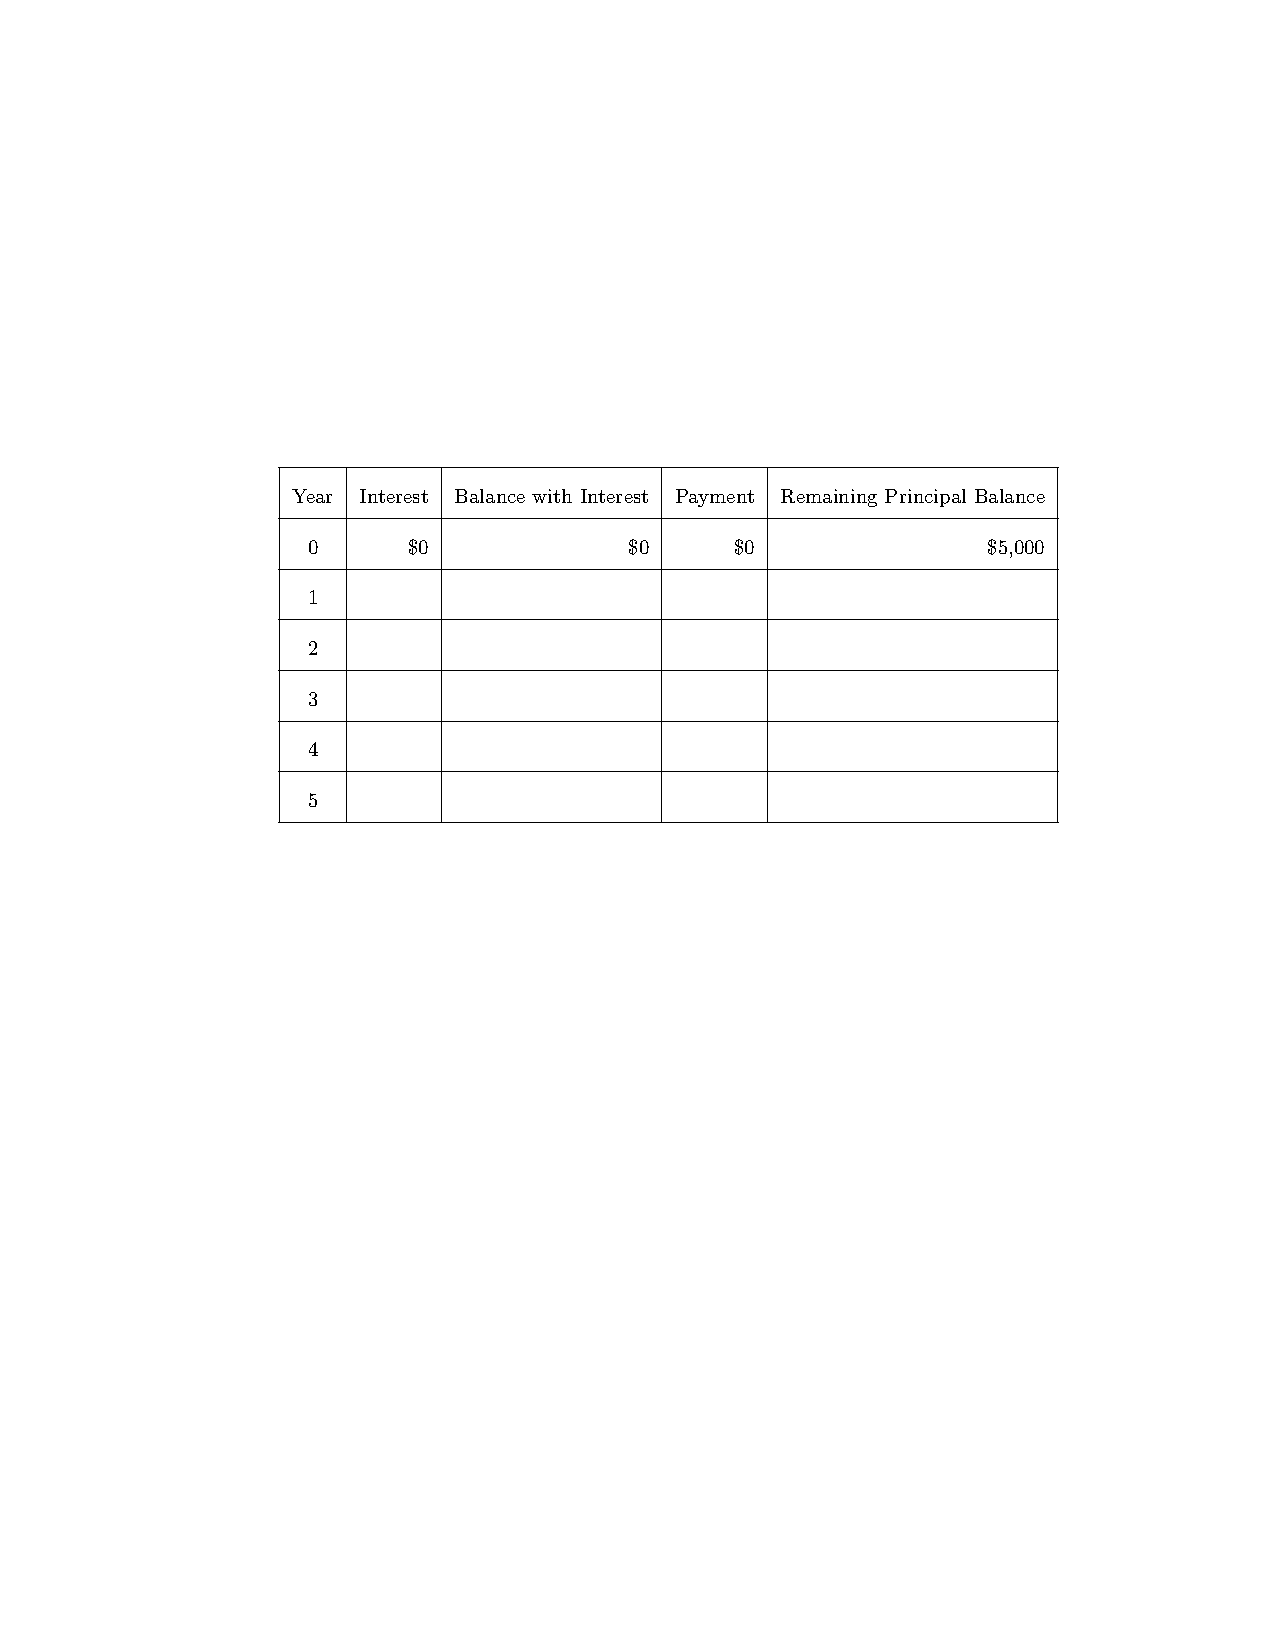
\includegraphics[scale=3]{payingOffDebtTableGraphic.pdf}
% \end{image}
\end{question}

\begin{question}
Based on your table, was your guess is too low, too high, or just
right?  
\begin{multipleChoice}
  \choice[correct]{Too low}
  \choice{Too high}
  \choice{Just right}
\end{multipleChoice}
\vfill
\begin{question}
Correct!  The remaining principal balance is still \wordChoice{\choice[correct]{positive}\choice{negative}\choice{zero}} at the end of the term of the loan, when the loan is supposed to be paid off.  

Use the GeoGebra spreadsheet below to find (to the closest penny) better equal annual payments: 
\begin{center}
\geogebra{g4atuesr}{740}{300}
\end{center}
To the closest penny, the loan can be paid off in \emph{four (4)} years with a payment of $\answer{1692.07}$.  

Alternatively, the loan can be paid off in \emph{five (5)} years, with equal annual payments of $\answer{1385.85}$ (again to the closest penny).  

Note: Because loans payments cannot include partial pennies, the last scheduled payment is usually slightly different so that the final balance will be exactly $\answer{0}$.  
\end{question}
\end{question}

\section*{Federal Student Loans}
%\href{https://studentaid.gov/announcements-events/save-plan}
%\href{https://bidenwhitehouse.archives.gov/briefing-room/statements-releases/2023/10/04/president-biden-announces-an-additional-9-billion-in-student-debt-relief-for-125000-americans/}{Whitehouse press release}
Although the Supreme Court struck down the Biden administration's initial plan to provide broad debt relief of \$10{,}000 to most borrowers and \$20{,}000 to Pell Grant recipients, read this 
\href{https://bidenwhitehouse.archives.gov/briefing-room/statements-releases/2025/01/13/statement-from-president-joe-biden-on-approving-student-debt-cancellation-for-over-5-million-americans/}{Whitehouse press release} for a summary of what the Biden administration did instead.  
\begin{question}
The administration provided targeted debt relief to what categories of borrowers?  \emph{(Select all.)}
\begin{selectAll}
\choice{Borrowers from institutions in the Big-12, SEC, or from Michigan}
\choice[correct]{Borrowers in Public Service Loan Forgiveness programs}
\choice{Borrowers who are Wall Street traders or financial analysts}
\choice[correct]{Borrowers in income-driven repayment plans}
\choice[correct]{Borrowers who have total or permanent disabilities} 
\choice{Borrowers who are fisherman, farmers, or agricultural workers}
\choice[correct]{Borrowers who were cheated or otherwise defrauded by their institutions}
\end{selectAll}
\begin{question}
Correct!  Using existing law and regulations, the Biden-Harris Administration had approved debt cancellation for over $\answer{5}$ million borrowers.  

These programs still exist today, as described \href{https://studentaid.gov/manage-loans/forgiveness-cancellation}{here}, though it is not clear whether the current administration will be as proactive in identifying eligible borrowers.  


To address the ongoing problem of borrowers staying in repayment for decades, often owing more than what they borrowed, the Biden administration proposed a new \href{https://bidenwhitehouse.archives.gov/briefing-room/statements-releases/2023/08/22/fact-sheet-the-biden-harris-administration-launches-the-save-plan-the-most-affordable-student-loan-repayment-plan-ever-to-lower-monthly-payments-for-millions-of-borrowers/}{student loan repayment program}.  Although this program was on hold due to legal challenges, and was discontinued by the current administration, 
answer the questions below based on what was proposed.  

\begin{question}
What was the acronym for the proposed student loan repayment program?  $\answer[format=string]{SAVE}$
\begin{question}
Correct!  Saving on a Valuable Education (SAVE) was an IDR plan that reduced payments on undergraduate loans from $10\%$ to $\answer{5}\%$ of a borrower's
discretionary income.  

What does IDR stand for?  $\answer[format=string]{Income-driven repayment}$.  Hint: 3 words, with a hyphen. 

The SAVE plan defined a borrower's ``discretionary income'' as the difference between their AGI and $\answer{225}\%$ of the U.S. Department of Health and Human Services Poverty Guideline amount for their family size.  

What does AGI stand for?  $\answer[format=string]{adjusted gross income}$. Hint: 3 words. 

Furthermore, the SAVE Plan had an \emph{interest benefit}: If you made your full monthly payment, but it was not enough to cover the accrued monthly interest, which of the following would be true? \emph{(Select all.)} 
\begin{selectAll}
\choice{Your loan balance would get larger.}
\choice{Your next payment would need to be larger.}
\choice{The interest would be larger the following month.}
\choice[correct]{The government would not charge the rest of the interest that accrued that month.}
\choice[correct]{The SAVE Plan would prevent your balance from growing due to unpaid interest.}
\end{selectAll}
\end{question}
\end{question}
\end{question}
\end{question}


%
%\begin{question}%[0in]
%  %Complete the table again for other possible payment amounts until
%  %you have found the ``best'' annual payment.  %(In Ximera, enter just
%  %the last row of your table.)
%
%  Complete the table again for a payment
%  of $\$1219.45$.  Round all answers to the nearest cent.
%  \[
%  \begin{array}{|c|c|c|c|c|}
%    \hline
%    \text{Year} & \text{Interest}             & \text{Balance with Interest} & \text{Payment}    & \text{Remaining Principal Balance}\\ \hline
%    0  & \$ 0               & ---                   & \$ 0        & \$ 5000 \\ \hline
%    1  & \$ \answer[tolerance=0]{350}    & \$ \answer[tolerance=0]{5350}    & \$ 1219.45  & \$ \answer[tolerance=0]{4130.55} \\ \hline
%    2  & \$ \answer[tolerance=0]{289.14} & \$ \answer[tolerance=0]{4419.69} & \$ 1219.45  & \$ \answer[tolerance=0]{3200.24} \\ \hline
%    3  & \$ \answer[tolerance=0]{224.02} & \$ \answer[tolerance=0]{3424.26} & \$ 1219.45  & \$ \answer[tolerance=0]{2204.81} \\ \hline
%    4  & \$ \answer[tolerance=0]{154.34} & \$ \answer[tolerance=0]{2359.15} & \$ 1219.45  & \$ \answer[tolerance=0]{1139.70} \\ \hline
%    5  & \$ \answer[tolerance=0]{79.78}  & \$ \answer[tolerance=0]{1219.48} & \$ 1219.45  & \$ \answer[tolerance=0]{0.03} \\ \hline
%    \end{array}
%  \]
%
%%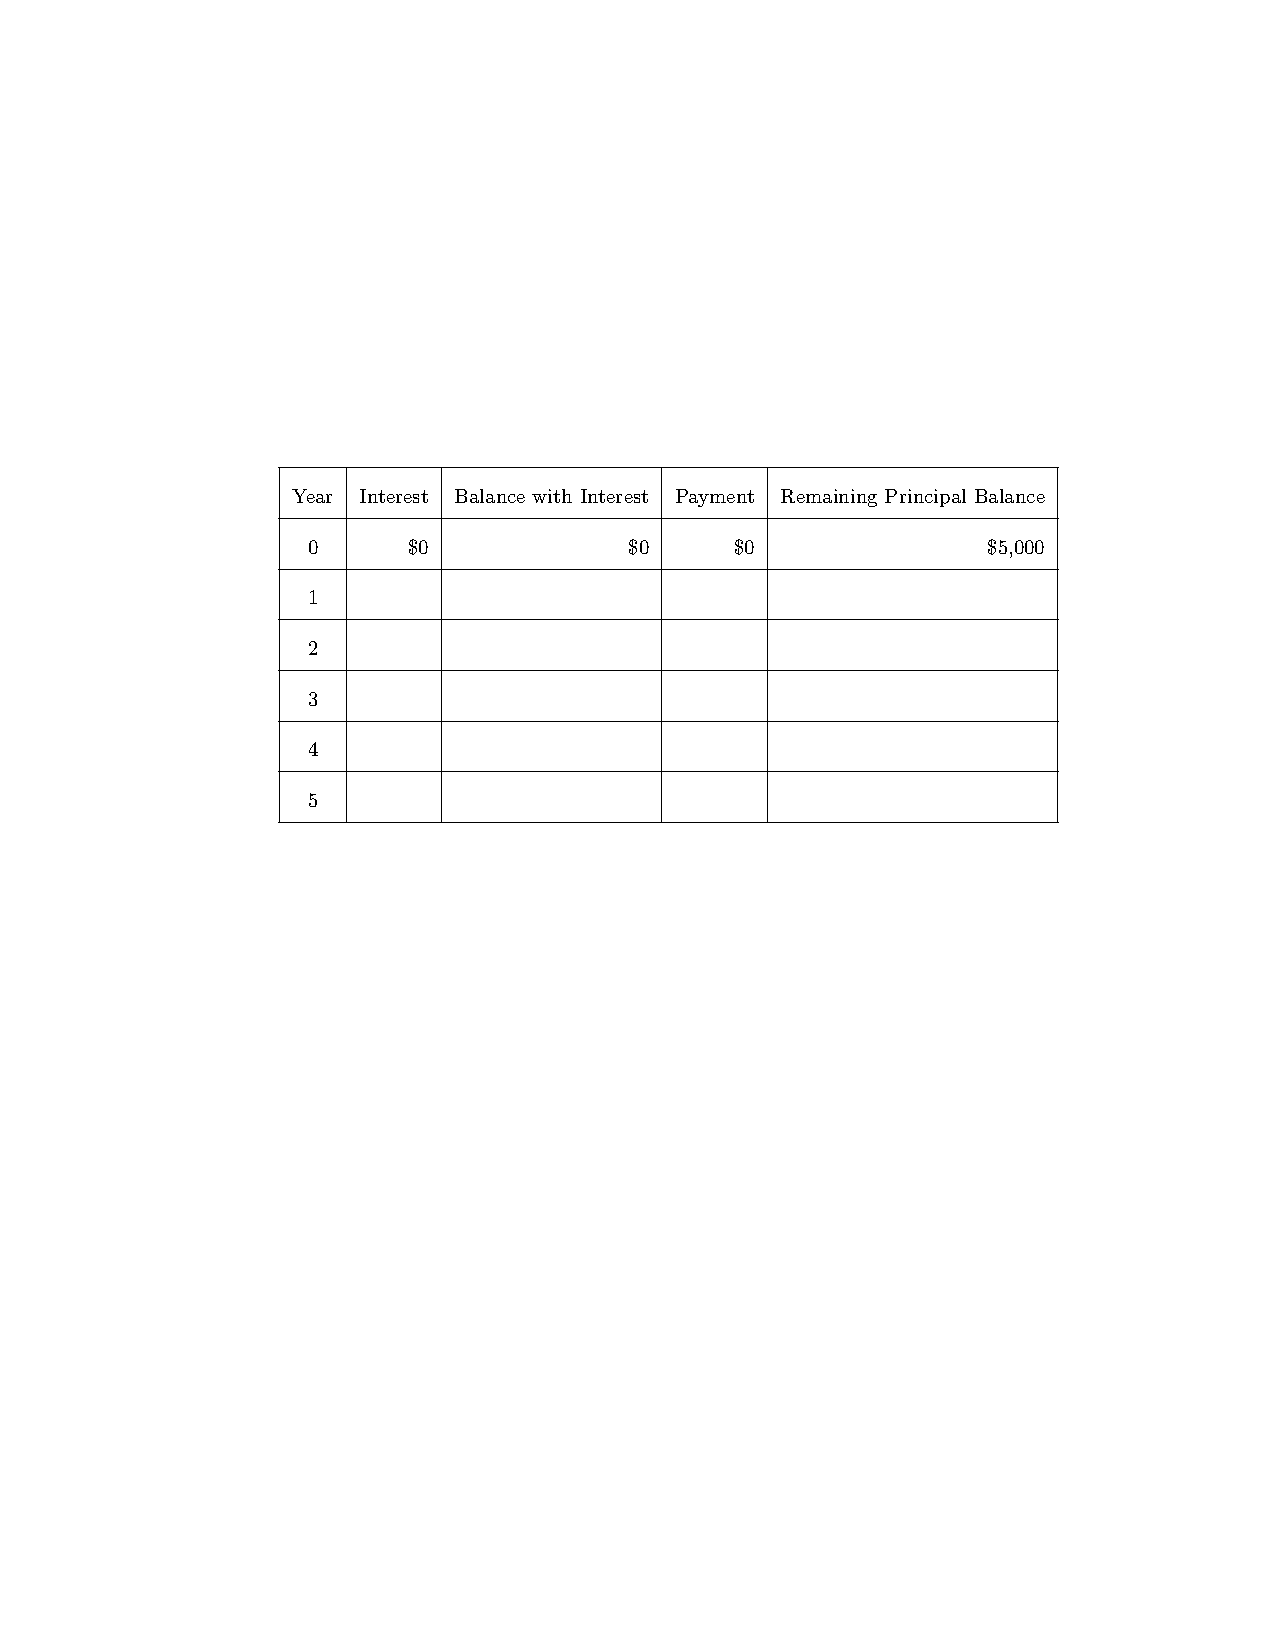
\includegraphics{payingOffDebtTableGraphic.pdf}
%\end{question}
%
%\begin{question}
%Using your best annual payment, how much interest would you pay in total over the $5$ years? 
%\begin{prompt}
%  You would pay \$ $\answer[tolerance=0]{1097.28}$.
%\end{prompt}
%\end{question}
%
%%% \begin{question}[.5in]
%%% Complete the table again, this time with a beginning principal of $P$, an interest rate of $r$,
%%% and a payment amount of $x$.  Hint: It helps to collect factors of $(1+r)$.
%
%%% Then write an equation that must be true if $x$ is the correct
%%% payment amount.   %(In Ximera, enter just the equation.)
%
%%% 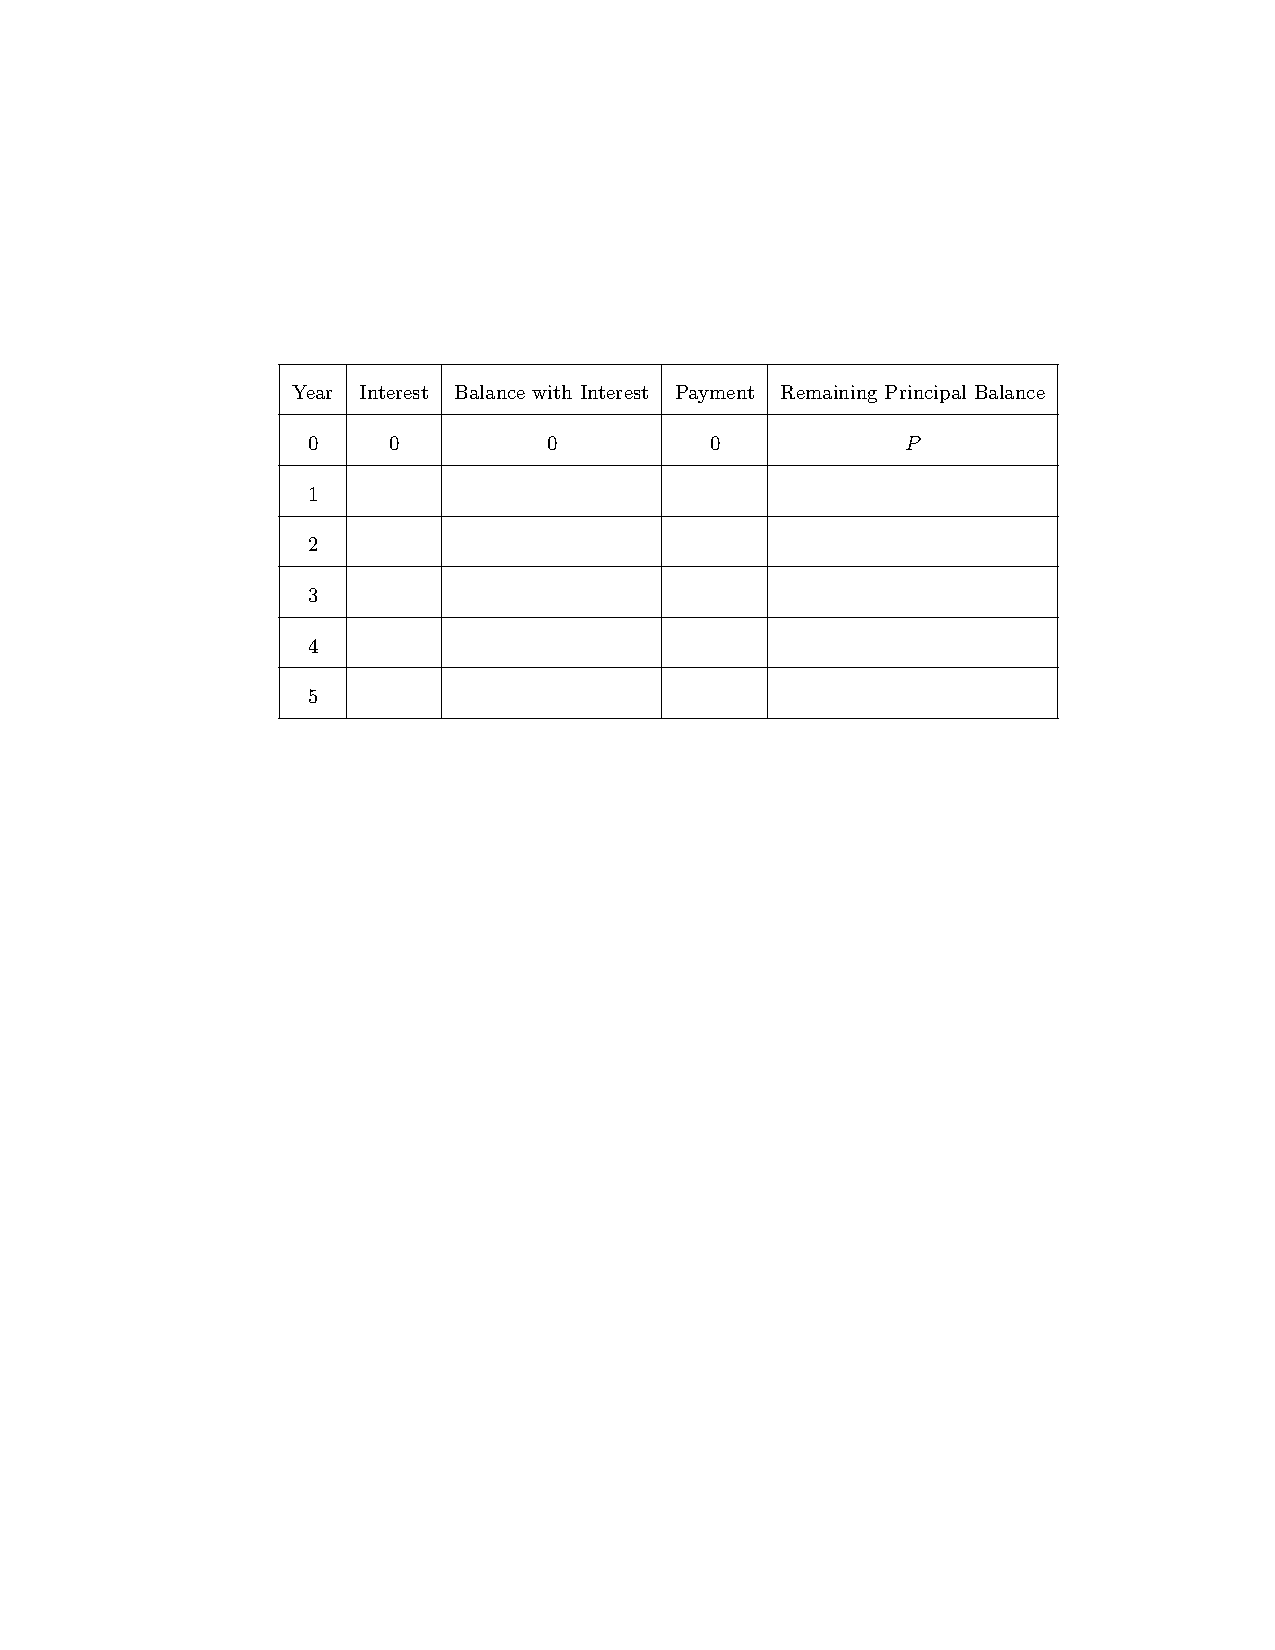
\includegraphics{payingOffDebtTableGraphic2.pdf}
%
%%% \begin{freeResponse}
%%% \end{freeResponse}
%%% \end{question}
%
%%% \begin{question}
%%% What is your next question?   
%%% \begin{freeResponse}
%%% \end{freeResponse}
%%% \end{question}
%
%
%%\begin{question}
%%Some students notice that the equation above includes a geometric series.  Write the geometric series here.
%%\begin{freeResponse}
%%\end{freeResponse}
%%\end{question}
%%
%%\begin{question}
%%How do you know this is a series?  How do you know this is a geometric series?   
%%\begin{freeResponse}
%%\end{freeResponse}
%%\end{question}
%%
%%\begin{question}
%%Call the geometric series $S$, and note that if you multiply $S$ by $1.07$, the ``common ratio,'' you get another geometric series with many of the same terms.  Use these observations to find the sum of the series.   
%%\begin{freeResponse}
%%\end{freeResponse}
%%\end{question}


\end{document}
